%!TEX root = ../dokumentation.tex

\chapter{Systemdokumentation}

Klare Beschreibung des entwickelten System\\
Konzeptbestandteile:\\
Zielsetzung\\
Benutzer(gruppen)/ Stakeholder\\
funktionale / qualitative / organisationale Anforderungen\\
aussagekräftiges Architekturmodell\\
technische Umsetzung\\
etc.\\
\\
Alternativen erwähnen\\
Abwägungen\\
Begründungen\\
Abweichungen vom Konzept anführen und begründen\\
Elementare Klassen \& Methoden\\
Fokus / roter Faden erkenn- und nachvollziehbar\\


\newpage

%!TEX root = ../dokumentation.tex

\section{Allgemeines}



\newpage

%!TEX root = ../dokumentation.tex

\section{Bearbeitung der Proof of Concepts}

\newpage

%!TEX root = ../dokumentation.tex

\section{POC1}




\newpage

%!TEX root = ../dokumentation.tex

\section{POC2}





\newpage

\newpage

%!TEX root = ../dokumentation.tex

\section{Entwickeltes System}


\subsection{Android Client}

\subsection{Activities}


\begin{figure}[H]
	\centering
	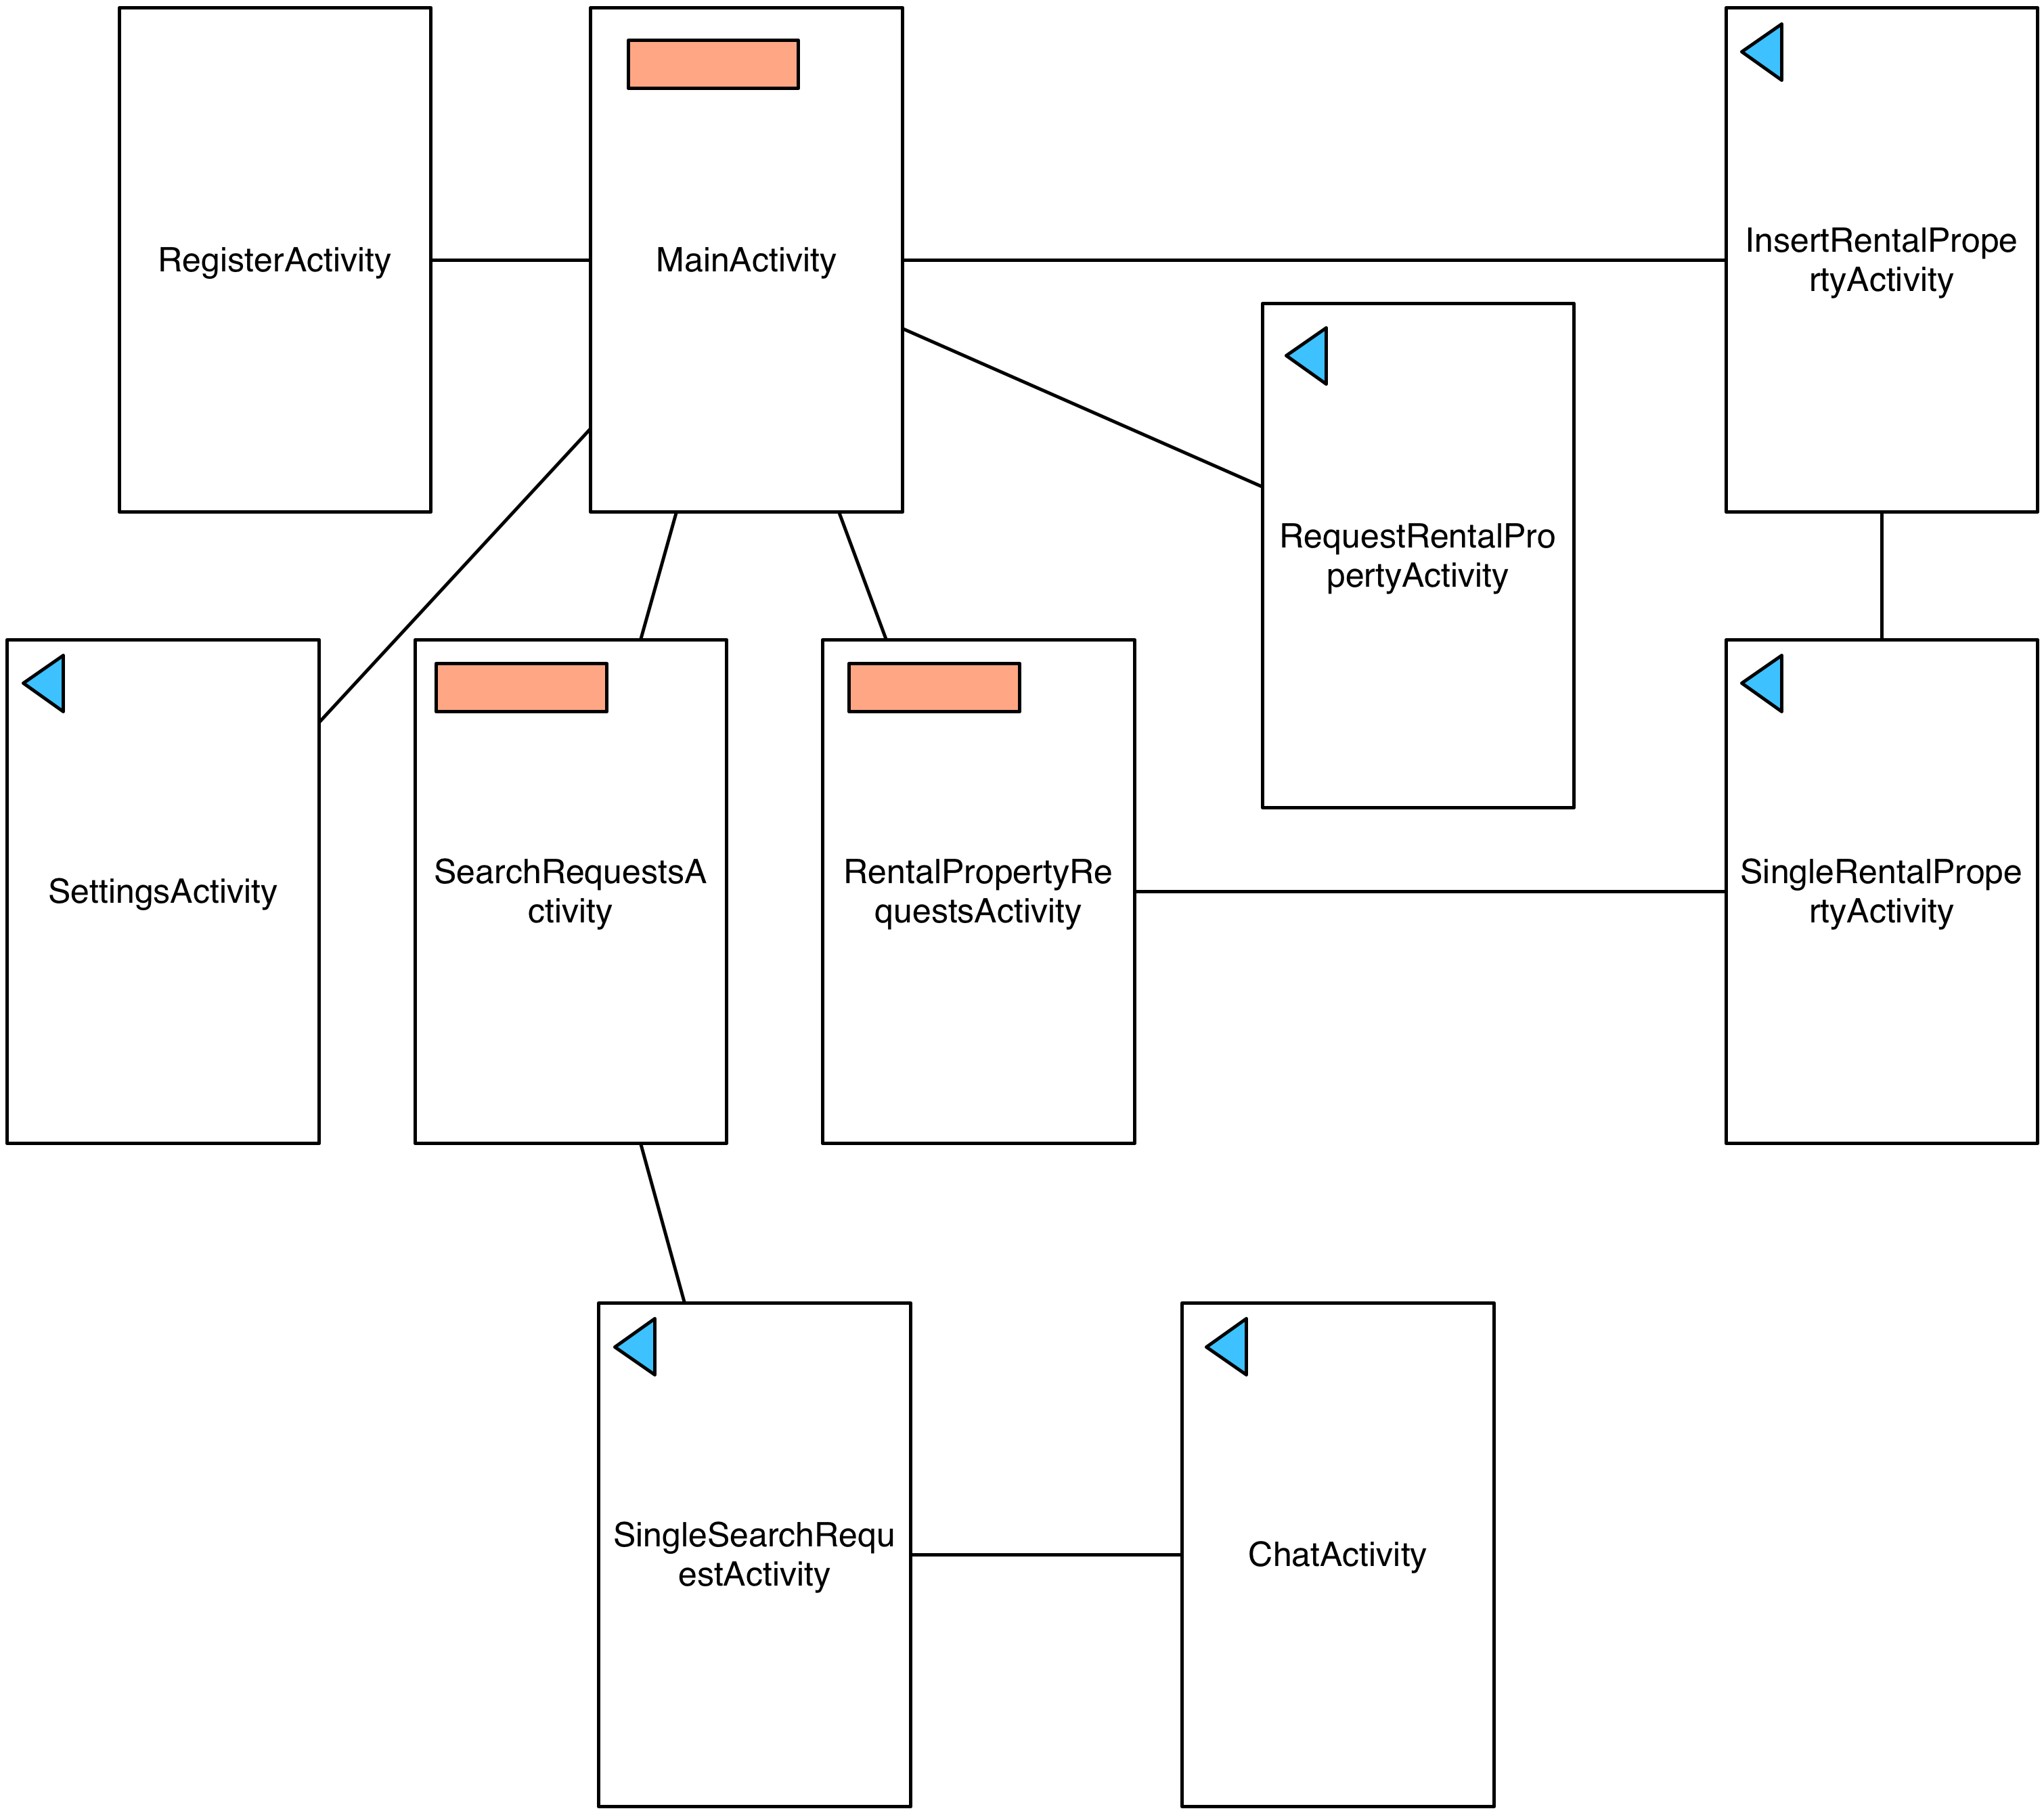
\includegraphics[width=0.85\textwidth]{./images/activitiesoverview.png}
	\caption{Übersicht der Activities und Navigationselementen}
	\label{fg:activitiesoverview}
\end{figure}


\subsection{Datenbank}

Wie im Proof-of-Concept „Lokale Datenbankanbindung“ (vgl Kapitel 3.2.4) bereits dokumentiert, wird das System mit dem Datenbanksystem SQLite arbeiten. Im Folgenden wird nun auf die endgültige Implementierung im System eingegangen.

Zunächst wurde eine abstrakte Klasse „Table“ entwickelt (Code \ref{ls:abstracttableclass}), welches nichts anders macht, als den Datenbanknamen sowie die aktuelle Datenbankversion beinhaltet. Die Klasse erweitert die Klasse „SQLiteOpenHelper“.

\begin{lstlisting}[label=ls:abstracttableclass,caption=Abstrakte Klasse „Table“]
public abstract class Table extends SQLiteOpenHelper {
	private static final String DATABASE_NAME = "data.db";
	private static final int DATABASE_VERSION = 1;

	public Table(Context context) {
		super(context, DATABASE_NAME, null, DATABASE_VERSION);
	}
}
\end{lstlisting}

Der Ausschnitt (Code \ref{ls:userstableclass}) der Implementation der „UserTable“ demonstriert die Vererbung der Klasse „Table“.

\begin{lstlisting}[label=ls:userstableclass,caption=Ausschnitt aus der Klasse „UsersTable“]
public class UsersTable extends Table {

	public static final String TABLE_NAME = "users";
	public static final String COLUMN_NAME_ID = "id";
	public static final String COLUMN_NAME_USER_NAME = "name";

	private static final String TABLE_CREATE =
		"CREATE TABLE " + TABLE_NAME + " (" +
			COLUMN_NAME_ID + " integer primary key autoincrement," +
			COLUMN_NAME_USER_NAME + " text NOT NULL" +
		");";

	private static final String TABLE_DROP =
		"DROP TABLE IF EXISTS " + TABLE_NAME;

	public UsersTable(Context context) {
		super(context);
	}

	public void onCreate(SQLiteDatabase db) {
		db.execSQL(TABLE_CREATE);
	}
}
\end{lstlisting}

Hierbei hat sich als hilfreich erwiesen, Tabellenspezifische Angaben wie Tabellenname oder Spaltenamen in Konstanten auszulagern, um diese wiederverwertbar zu gestalten. Dies spiegelt sich zum Beispiel bei einem Insert-Befehl wieder (Code \ref{ls:userstableinsert}) .

\begin{lstlisting}[label=ls:userstableinsert,caption=Exemplarisches Insert in die „UsersTable“]
UsersTable usersTable = new UsersTable(this);
SQLiteDatabase usersTableDb = usersTable.getWritableDatabase();

ContentValues values = new ContentValues();
values.put(UsersTable.COLUMN_NAME_ID, id);
values.put(UsersTable.COLUMN_NAME_USER_NAME, username);

long userId = usersTableDb.insert(
	UsersTable.COLUMN_NAME_ID,
	UsersTable.COLUMN_NAME_USER_NAME,
	values);
\end{lstlisting}

\subsection{Serveranwendung}

\subsection{Datenbank}

Für die Speicherung von Daten wurden die Datenbanksysteme SQLite, MySQL und MongoDB in Erwägung gezogen. Die Einbindung in Java geschieht dabei über Treiber. Der zugehörige Treiber  muss dafür geladen werden und dem Projekt als Bibliothek zugewiesen werden.

Bei der Implementierung ist auf einen Fehler einzugehen: Das Laden des Laden des Treibers wird über einen dynamischen Klassenaufruf gesteuert. In den jeweiligen Anleitungen war folgender Schnipsel (Code \ref{ls:wrongdriveruse}) zu sehen (vgl. Verbindung mit MySQL über die Schnittstelle DriverManager\footnote{http://dev.mysql.com/doc/refman/5.1/de/connector-j-usagenotes-basic.html\#connector-j-usagenotes-connect-drivermanager})

\begin{lstlisting}[label=ls:wrongdriveruse,caption=Fehlerhafter dynamischer Klassenaufruf]
try {
	Class.forName("com.mysql.jdbc.Driver").newInstance();
} catch (Exception ex) {
	// Fehler behandeln
}
\end{lstlisting}

Die Nutzung des Schnipsels gab jedoch nicht das gewünschte Ergebnis aus, genauer gesagt gar nichts. Die Lösung des Problems bestand darin, den Aufruf \textit{.newInstance()} zu entfernen (Code \ref{ls:correctdriveruse}).

\begin{lstlisting}[label=ls:correctdriveruse,caption=Korrekter dynamischer Klassenaufruf]
try {
	Class.forName("com.mysql.jdbc.Driver")
} catch (Exception ex) {
	// Fehler behandeln
}
\end{lstlisting}

In der folgenden Übersicht werden die drei Datenbanksysteme anhand eines Beispiels - anlegen einer Tabelle und einfügen eines Wertes - gegenübergestellt:

\subsubsection{SQLite}

Treiber: \url{https://bitbucket.org/xerial/sqlite-jdbc}
\begin{lstlisting}[label=ls:mysqlexample,caption=Exemplarische Darstellung der Nutzung des SQLite Treibers]
Class.forName("org.sqlite.JDBC");
Connection connection = DriverManager.getConnection("jdbc:sqlite:findyourcamp.db");
Statement statement = con.createStatement();
statement.executeUpdate("drop table if exists users");
statement.executeUpdate("create table users (id integer, name string)");
statement.executeUpdate("insert into person values(1, 'max')");
\end{lstlisting}

\subsubsection{MySQL}

Treiber: \url{http://dev.mysql.com/downloads/connector/j/}
\begin{lstlisting}[label=ls:mysqlexample,caption=Exemplarische Darstellung der Nutzung des MySQL Treibers]
Class.forName("com.mysql.jdbc.Driver");
Connection connection = DriverManager.getConnection("jdbc:mysql://localhost:3306/findyourcamp", "username", "password");
Statement statement = con.createStatement();
statement.executeUpdate("drop table if exists users");
statement.executeUpdate("create table users (id int, name text)");
statement.executeUpdate("insert into person values(1, 'max')");
\end{lstlisting}

\subsubsection{MongoDB}

Treiber: \url{http://docs.mongodb.org/ecosystem/drivers/java/}
\begin{lstlisting}[label=ls:mongoexample,caption=Exemplarische Darstellung der Nutzung des MongoDB Treibers]
MongoClient mongoClient = new MongoClient();
DB db = mongoClient.getDB("findyourcamp");
DBCollection collection = db.getCollection("users");
collection.insert(new BasicDBObject("name", "max"));
\end{lstlisting}

SQLite kennen wir schon aus der Entwicklung der Android Applikation. Als weiteres relationales Datenbanksystem ist MySQL gewählt worden. Der Unterschied zwischen beiden System liegt darin, dass MySQL auf eine exterene Datenbasis setzt, wo SQLite sich direkt in die Anwendungen integrieren lässt. MongoDB hingegen kommt aus der NoSQL Sparte. Die Daten werden im JSON Format hinterlegt, wodurch das System gut skalierbar ist. Die Nachteile liegen allerdings in der fehlenden Relationen oder einer Volltext-Suche.

In den Tests (Code \ref{ls:performancetest}) zeigte sich außerdem, dass NoSQL, sowie auch SQLite, um 50\% langsamer als die MySQL Implementation war.

\begin{lstlisting}[label=ls:performancetest,caption=Perfomancetest zwischen MySQL und SQLite,language=bash]
$ time java -jar test_sqlite.jar
java -jar test_sqlite.jar 2,24s user 0,46s system  97% cpu 2,760 total
$ time java -jar test_mysql.jar
java -jar test_mysql.jar  1,47s user 0,17s system 133% cpu 1,225 total
\end{lstlisting}

Da der Zeitfaktor doch eine große Rolle in unserem System spielt, wurde entschieden für die Serveranwendung auf MySQL zu setzen. Jedoch sollte, sofern es die Zeit zulässt, eine gewisse Abstraktion geschaffen werden, wodurch ein späteres Ändern des Datenbanksystems durchführbar ist.

\subsection{Matching Algorithmus}

Erst Location, dann gruppengröße, dann preis, dann BooleanFeatures



\newpage





